\chapter{Implementacja}
W niniejszym rozdziale przedstawiona zostanie szczegółowa analiza aspektów technicznych związanych z implementacją aplikacji. Na początku zaprezentowane zostaną wykorzystane narzędzia wraz z uzasadnieniem ich wyboru w kontekście wymagań projektowych. Następnie omówiona zostanie architektura warstw systemu. W dalszej części rozdziału szczegółowo opisane zostaną poszczególne moduły systemu oraz ich wzajemne powiązania. Następna część poświęcona będzie omówieniu implementacji kluczowych funkcjonalności: mechanizmu publikacji ogłoszeń, modułu wizualizacji tras na mapie oraz algorytmu rekomendacji ogłoszeń. W ostatniej części rozdziału przedstawione zostanie podejście do testowania aplikacji oraz proces jej wdrożenia na środowisko produkcyjne.

\section{Opis narzędzi}
Aplikacja została wykonana w technologii webowej, przy użyciu fullstackowego frameworka \texttt{Next.js} \cite{Next} (w wersji \texttt{15.1.3}). Jest to popularny sposób tworzenia aplikacji webowych, zapewniający wiele przydatnych funkcji poprawiających optymalizacje. Między innymi \texttt{Next.js} skraca czas potrzebny do załadowania aplikacji poprzez renderowanie kodu \texttt{HTML} strony, już podczas kompilacji aplikacji. Został on oparty na innym frameworku - React \cite{React}, jest to jedna z najpopularniejszych bibliotek \texttt{JavaScript} do budowania interfejsów użytkownika. Opiera się on na koncepcji komponentów - niezależnych, wielokrotnego użytku bloków interfejsu. Komponenty te w  \texttt{Next.js} są renderowane po stronie serwera, co znacząco przyspiesza pierwsze ładowanie strony. Dodatkowo renderowanie komponentów aplikacji po stronie serwera, pozytywnie wpływa na algorytmy \texttt{SEO}, co skutkuje lepszym pozycjonowaniem serwisu w wyszukiwarkach internetowych. \texttt{Next.js} posiada zintegrowane rozwiązanie fullstackowe, oznacza to, że zarówno backend jak i frontend aplikacji wykorzystują tę samą bazę kodu. Takie podejście znacząco upraszcza proces developmentu i utrzymania aplikacji, eliminując potrzebę zarządzania oddzielnymi projektami dla części serwerowej i klienckiej. Dodatkowo ułatwia proces wdrożenia aplikacji na środowisko produkcyjne.

Zamiast standardowych klas \texttt{CSS}, do interfejsu użytkownika została użyta biblioteka \texttt{Tailwind} \cite{Tailwind} (w wersji \texttt{3.4.1}). Jest to narzędzie typu \texttt{utility-first CSS}, które pozwala na szybkie tworzenie responsywnych interfejsów poprzez zastosowanie predefiniowanych klas bezpośrednio w kodzie HTML.

Do wyświetlania na mapie tras z ogłoszeń, użyte zostało \texttt{API Leaflet}. Jest to darmowy serwis oferujący interaktywne mapy, który umożliwia łatwą implementację funkcjonalności takich jak wyświetlanie markerów, rysowanie tras czy obsługa zdarzeń związanych z interakcją użytkownika z mapą. Biblioteka została zoptymalizowana pod kątem urządzeń mobilnych, zapewniając płynne działanie i responsywność na różnych rozmiarach ekranów.

Testy jednostkowe aplikacji wykonane zostały przy użyciu biblioteki \texttt{Jest} \cite{Jest} (w wersji \texttt{29.7.0}). Framework ten został wybrany ze względu na jego natywną integrację z \texttt{Next.js} oraz możliwość łatwego tworzenia i uruchamiania testów dla komponentów React.

W celu usprawnienia procesu wdrożenia aplikacji na środowisko produkcyjne, zastosowano narzędzie \texttt{Docker} \cite{Docker}. Technologia ta pozwala na izolację poszczególnych modułów aplikacji w dedykowanych kontenerach, zapewniając jednakowe środowisko uruchomieniowe niezależnie od platformy. Kontenery \texttt{Docker} stanowią wyizolowane, lekkie maszyny wirtualne, w których uruchamiana jest aplikacja. Zastosowanie takiej architektury umożliwia zdefiniowanie wszystkich wymaganych zależności na etapie budowania obrazu kontenera, eliminując konieczność ich konfiguracji w środowisku produkcyjnym.

\section{Opis architektury}
TODO
\subsection{Architektura warstw}
\begin{figure}[H]
	\centering
		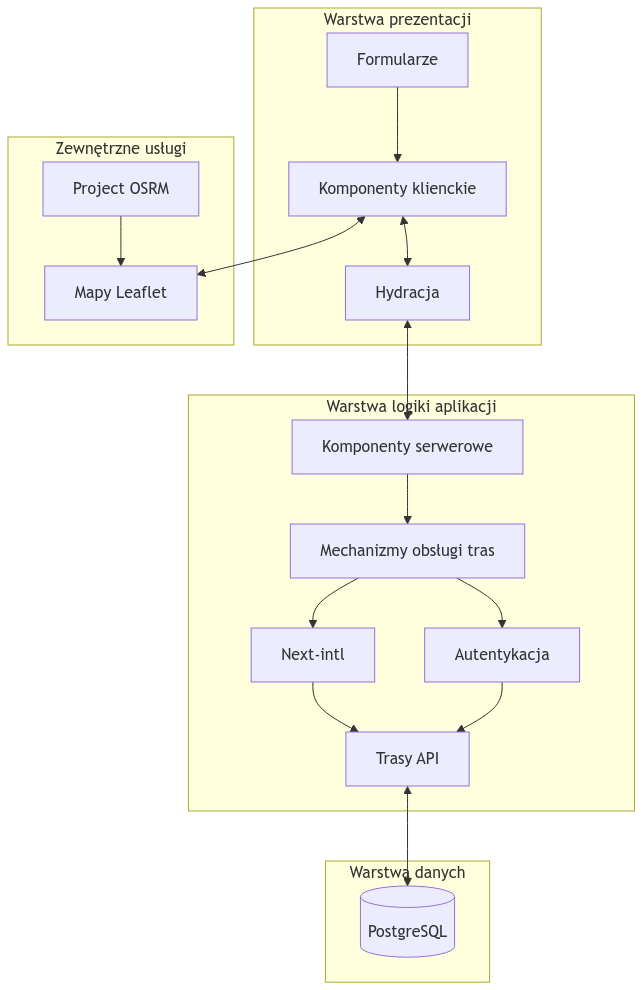
\includegraphics[width=0.7\linewidth]{rozdzial2/diagram_warstw.png}
	\caption{Diagram architektury warstw aplikacji}
	\label{Diagram warstw}
\end{figure}
Powyższy diagram przedstawia architekture warstw aplikacji. Zostały na nim wyszczególnione następujące warstwy:
\begin{enumerate}
    \item \textbf{Warstwa prezentacji} - odpowiada za bezpośrednią interakcje z użytkownikiem. W jej skład wchodzą:
    \begin{enumerate}
        \item formularze - stanowią pośrednika między użytkownikiem, a warstwą logiki aplikacji. Pozwalają na wysyłanie wprowadzonych danych do warstwy logiki aplikacji,
        \item komponenty klienckie (ang. \emph{client components}) - interaktywne elementy interfejsu użytkownika renderowane po stronie przeglądarki końcowego użytkownika, które:
        \begin{itemize}
            \item obsługują zdarzenia użytkownika (kliknięcia, wprowadzanie danych),
            \item zarządzają stanem lokalnym aplikacji przy użyciu \emph{React hooks},
            \item implementują dynamiczne zachowania interfejsu bez przeładowywania strony,
            \item komunikują się z API poprzez żądania HTTP,
            \item renderują interaktywne elementy mapy przy użyciu biblioteki Leaflet.
        \end{itemize}
        \item hydracja - kluczowy proces w architekturze aplikacji \texttt{Next.js}. Przekształca początkowy, statyczny widok strony w pełni interaktywną aplikację React. Poprzez wypełnianie komponentów klienckich danymi pozyskanymi z warstwy logicznej aplikacji.
    \end{enumerate}
    \item \textbf{Warstwa logiki aplikacji} - są w niej zawarte wszelkie mechanizmy, do których użytkownik końcowy nie może mieć wglądu z uwagi na bezpieczeństwo. Warstwa ta składa się z:
    \begin{enumerate}
        \item komponentów serwerowych (ang. \emph{server components}) - komponenty intefejsu użytkownika, które:
        \begin{itemize}
            \item są renderowane po stronie serwera, a użytkownikowi zwracany jest gotowy kod HTML,
            \item redukują ilość JavaScript przesyłanego do przeglądarki,
            \item mogą bezpośrednio komunikować się z bazą danych,
            \item mają dostęp do wrażliwych danych i zmiennych środowiskowych,
            \item są odpowiednie do renderowania statycznej zawartości i elementów niewymagających interaktywności.
        \end{itemize}
        \item mechanizmów obsługi tras (ang. \emph{route handlers}) - odpowiadają za przetwarzanie żądań przychodzących i wysyłanie odpowiedzi.
        \begin{itemize}
            \item obsługują metody HTTP (\emph{GET, POST, PUT, DELETE}),
            \item zapewniają bezpieczną komunikację między frontendem a backendem aplikacji.
        \end{itemize}
        \item Next-intl - biblioteka do internalizacji, jest ona wykorzystywana do prezentacji treści w różnych językach (polskim, angielskim oraz niemieckim).
        \item Autentykacja - zapewnia bezpieczeństwo poprzez blokowanie wybranych tras API nieautoryzowanym użytkownikom.
        \item Trasy API - specjalne endpointy w aplikacji, są wykorzystywane do:
        \begin{itemize}
            \item zarządzania ogłoszeniami (dodawanie, zatwierdzanie, usuwanie zleceń),
            \item obsługi procesu rejestracji i logowania użytkowników,
            \item pobierania i filtrowania listy dostępnych ogłoszeń,
            \item komunikacji z zewnętrznym API OSRM dla wyznaczania tras,
        \end{itemize}
    \end{enumerate}
    \item \textbf{Warstwa danych} - warstwa odpowiadająca za przechowywanie oraz dostarczanie wszelkich danych aplikacji. W aplikacji wykorzystano relacyjną bazę danych PostgreSQL, która przechowuje informacje o:
    \begin{enumerate}
        \item użytkownikach systemu i ich rolach,
        \item zleceniach transportowych i ich statusach,
        \item lokalizacjach geograficznych (punkty początkowe i końcowe tras),
        \item czatach między użytkownikami oraz umowami zawartymi między nimi,
    \end{enumerate}
    \item \textbf{Zewnętrzne usługi} - systemy i API wykorzystywane do rozszerzenia funkcjonalności aplikacji:
    \begin{enumerate}
        \item Project OSRM (ang. \emph{Open Source Routing Machine}), używany jest do zapewnia funkcji wyznaczania tras między punktami. Oferuje API do integracji z aplikacjami transportowymi.
        \item Mapy Leaflet, jest to biblioteka służąca do interaktywnej wizualizacji map, która umożliwia wyświetlanie markerów lokalizacji. Pozwala również na rysowanie tras na mapie oraz zapewnia intuicyjną nawigację i przybliżanie mapy.
    \end{enumerate}
\end{enumerate}

\section{Opis implementacji}
W tym podrozdziale zostały opisane implementacje funkcjonalności mechanizmu publikacji ogłoszeń, modułu wizualizacji tras na mapie oraz algorytmu rekomendacji ogłoszeń.

\subsection{Implementacja mechanizmu publikacji ogłoszeń o planowanej trasie}
Dodawanie nowego ogłoszenia o planowanej trasie odbywa się poprzez wysłanie przez użytkownika wypełnienionego formularza. W bazie danych muszą zostać zawarte informacje o adresie początkowym, adresie końcowym, datach odjazdu i przyjazdu, tytule ogłoszenia oraz jego opisie, a także o ładowności pojazdu (maksymalny ciężar towaru, maksymalne wymiary towaru oraz maksymalna wysokość towaru). Walidacja wprowadzonych przez użytkownika danych odbywa się po stronie serwera. Poniżej zamieszczony został fragment funkcji dodającej do bazy danych nowe ogłoszenie o planowanej trasie.

{\belowcaptionskip=-9pt
\begin{lstlisting}[language=JavaScript,caption=Wstępna walidacja danych przed dodaniem ogłoszenia do bazy danych, label=lst:addAnnouncement]
export async function addAnnouncement(state: NewAnnouncementFormState, formData: FormData) {
  const t = await getTranslations('addPost');
  const validatedFields = newAnnouncementSchema(t).safeParse({
    title: formData.get('title'),
    brand: formData.get('brand'),
    model: formData.get('model'),
    maxWeight: formData.get('maxWeight'),
    maxSize: formData.get('maxSize'),
    maxHeight: formData.get('maxHeight'),
    fromCity: formData.get('fromCity'),
    toCity: formData.get('toCity'),
    departureDate: formData.get('departureDate'),
    arrivalDate: formData.get('arrivalDate'),
    desc: formData.get('desc'),
    from: JSON.parse(formData.get('from') as string) as Address,
    to: JSON.parse(formData.get('to') as string) as Address,
  });
  if (!validatedFields.success) {
    return {
      errors: validatedFields.error.flatten().fieldErrors,
    };
  }
  // Dalszy fragment funkcji
}
\end{lstlisting}
}

W powyższym fragmencie funkcji \texttt{addAnnouncement} widoczny jest mechanizm dodawania nowego ogłoszenia o planowanej trasie. Funkcja realizuje kilka kluczowych zadań:
\begin{enumerate}
    \item \textbf{Walidacja danych wejściowych} - funkcja wykorzystuje schemat walidacji \texttt{newAnnouncementSchema} zdefiniowany przy pomocy biblioteki \texttt{Zod}. Do schematu podawana jako argument jest funkcja pobierająca tłumaczenia dla komunikatów błędów.
    \item \textbf{Obsługa danych} - dane są pobierane z obiektu \texttt{FormData}, dostarczanego podczas wysyłania formularza. Adresy początkowy i końcowy są parsowane z objektu \texttt{JSON} zawierającego dokładne informacje o współrzędnych, identyfikatorów krajów, stanów, miast, kodzie pocztowym oraz innych niezbędnych danych.
    \item \textbf{Mechanizm obsługi błędów} - w przypadku niepowodzenia walidacji funkcja zwraca do formularza obiekt z wyszczególnionymi błędami dla poszczególnych pól.
\end{enumerate}

Walidacja danych odbywa się po stronie serwera, jest to bezpieczniejszy sposób niż walidacja po stronie klienta, gdyż użytkownik końcowy nie ma wglądu w kod sprawdzający poprawność danych i nie może go obejść.

{\belowcaptionskip=-9pt
\begin{lstlisting}[language=JavaScript,caption=Schemat walidacji danych wejściowych, label=lst:addAnnouncementSchema]
export const newAnnouncementSchema = (t: any) =>
  z.object({
    title: z
      .string()
      .min(1, { message: t('mustNotBeEmpty') })
      .trim(),
    brand: z
      .string()
      .min(1, { message: t('mustNotBeEmpty') })
      .trim(),
    model: z
      .string()
      .min(1, { message: t('mustNotBeEmpty') })
      .trim(),
    maxWeight: z.coerce
      .number()
      .refine(inRange(1,50000), { message: t('valueBetween') + '1-50000' }),
    maxSize: z.string().regex(/^[1-9][0-9]*x[1-9][0-9]*$/, {
      message: t('formatIssue'),
    }),
    maxHeight: z.coerce
      .number()
      .refine(inRange(1, 1000), { message: t('valueBetween') + '1-1000' }),
    desc: z.string().trim(),
    departureDate: z.coerce.date(),
    arrivalDate: z.coerce.date(),
    from: AddressSchema(t),
    to: AddressSchema(t),
  });
\end{lstlisting}
}

Przedstawiony schemat walidacji danych wejściowych \texttt{newAnnouncementSchema} definiuje reguły sprawdzania poprawności dla nowego ogłoszenia transportowego przy użyciu biblioteki Zod. Schemat obejmuje następujące kluczowe elementy:
\begin{enumerate}
    \item \textbf{Walidacja tekstowa} - Pola takie jak tytuł, marka, model wymagają niepustej wartości, która jest dodatkowo przycinana z białych znaków.
    \item \textbf{Walidacja liczbowa} - Maksymalna waga towaru musi zawierać w zakresie 1-50000, a maksymalna wysokość towaru w zakresie 1-1000.
    \item \textbf{Walidacja formatu} - Maksymalny rozmiar towaru wymaga formatu \emph{szerokość} x \emph{wysokość} liczonych w europaletach (np. 3x2). Daty wyjazdu i przyjazdu są konwertowane do formatu daty.
    \item \textbf{Walidacja adresów} - wykorzystuje osobny schemat \texttt{AddressSchema} dla weryfikacji danych adresowych.
\end{enumerate}
Schemat używa funkcji tłumaczącej do generowania komunikatów błędów, co zapewnia internacjonalizację komunikatów walidacyjnych.

Jeżeli wprowadzone dane zostaną pozytywnie rozpatrzone przez walidacje, następuje dodanie ogłoszenia o planowanej trasie do bazy danych.

{\belowcaptionskip=-9pt
\begin{lstlisting}[language=JavaScript,caption=Dodawanie ogłoszenia do bazy danych, label=lst:addAnnouncementToDB]

export async function addAnnouncement(state: NewAnnouncementFormState, formData: FormData) {
    
    // Powyzej opisana walidacja danych

    const data = validatedFields.data;
    let [size_x, size_y] = data.maxSize.split('x').map(Number);
    const { userId } = await verifySession();
    
    const from_address_id = await addAddress(data.from);
    const to_address_id = await addAddress(data.to);
    
    await sql(
        'INSERT INTO announcements (title,description,start_date,arrive_date,max_weight,size_x,size_y,max_height,author_id,is_accepted,vehicle_brand,vehicle_model,from_address_id,to_address_id,road_color)VALUES($1,$2,$3,$4,$5,$6,$7,$8,$9,$10,$11,$12,$13,$14,$15)',
        [
        data.title,
        data.desc,
        data.departureDate,
        data.arrivalDate,
        data.maxWeight,
        size_x,
        size_y,
        data.maxHeight,
        userId,
        false,
        data.brand,
        data.model,
        from_address_id,
        to_address_id,
        '#' + ((Math.random() * 0xffffff) << 0).toString(16),
        ],
    );
    redirect({ locale: 'pl', href: '/announcements' });
}
\end{lstlisting}
}

Powyższy fragment funkcji \texttt{addAnnouncement} realizuje proces zapisu nowego ogłoszenia transportowego do bazy danych. Wykonwane są w nim następujące czynności:
\begin{enumerate}
    \item \textbf{Przygotowanie danych} - parsuje rozmiar towaru na osobne wartości \texttt{size\_x} i \texttt{size\_y}, a także weryfikuje czy użytkownik w rzeczywiście jest zalogowany. Następnie do tabeli \texttt{addresses} dodawane są rekordy z adresem początkowym oraz końcowym.
    \item \textbf{Zapis do bazy danych} - dodaje rekord do tabeli \texttt{announcements} używając wszystkich przesłanych przez użytkownika danych. Odbywa się to poprzez używanie zmiennych (\$1, \$2, ...), uodparnia to aplikacje na atak typu \texttt{SQL injection}.
    \item \textbf{Automatyczne przekierowanie do listy ogłoszeń po pomyślnym dodaniu}
\end{enumerate}
Domyślnie kolumna \texttt{is\_accepted} jest ustawiona na \texttt{false} ze względu na to, że ogłoszenie nie powinno być było widoczne publicznie natychmiast po dodaniu. Stanie się ono widoczne dopiero kiedy jeden z moderatorów je zatwierdzi. Wartość kolumny \texttt{road\_color} jest generowana losowo, kolor ten będzie używany do rysowania trasy przewozu na mapie.

\subsection{Implementacja wizualizacji tras na mapie}
W aplikacji użyto darmową open-source'ową biblioteke Leaflet, pozwala ona na wygenerowanie interaktywnej mapy, na której wyświetlane będą punkty oraz trasy. Wyświetlenie rzeczywistej trasy między punktami wymaga posiadania bazy danych ze współrzędnymi geograficznym wszystkich dróg na świecie. W aplikacji posłużono się gotowym darmowym rozwiązaniem w formie API. \texttt{Project OSRM} (ang. \emph{Open Source Routing Machine}) pozwala na wygenerowanie macierzy współrzędnych geograficznych, wskazujących na najkrótszą drogę między dwoma punktami.

{\belowcaptionskip=-9pt
\begin{lstlisting}[language=JavaScript,caption=Argumenty komponentu mapy, label=lst:mapProps]

export type Road = {
  from?: GeoPoint;
  to?: GeoPoint;
  postId?: string;
  color?: string;
};

type MapProps = {
  zoom?: number;
  className?: string;
  roads?: Road[];
};

export default function Map({ zoom = 13, className, roads = [] }: MapProps) {
// Dalszy fragment komponentu mapy
}
\end{lstlisting}
}

Komponent \texttt{Map} przyjmuje w argumencie wartość \texttt{zoom}, czyli poziom przybliżenia mapy, domyślnie w aplikacji ta wartość została ustawiona na 13, co daje nam widok na całą Europe. Argument \texttt{className} to klasy Tailwind, pozwala na stylizacje komponentu w zależności od potrzeb. Ostatni argument \texttt{roads} to tablica typu \texttt{Road}, typ ten zawiera informacje o trasie, współrzędnych geograficznych punktu początkowego oraz końcowego, identyfikator powiązanego z nią ogłoszenia oraz kolor rysowanej na mapie trasy.

{\belowcaptionskip=-9pt
\begin{lstlisting}[language=JavaScript,caption=Pobieranie najkrótszych tras między punktami, label=lst:fetchRoutes]
export default function Map({ zoom = 13, className, roads = [] }: MapProps) {
    
    const [routesPoints, setRoutesPoints] = useState<[number, number][][]>([]);
    const [selectedRoute, setSelectedRoute] = useState<number | null>(null);
    const t = useTranslations('map');

    useEffect(() => {
        const fetchRoutes = async () => {
        const newRoutes: [number, number][][] = [];
    
        for (const road of roads) {
            if (!road.from?.coordinates || !road.to?.coordinates) continue;
    
            try {
            const response = await fetch(
                `https://router.project-osrm.org/route/v1/driving/${road.from.coordinates[1]},${road.from.coordinates[0]};${road.to.coordinates[1]},${road.to.coordinates[0]}?overview=full&geometries=geojson`,
            );
    
            const data = await response.json();
    
            if (data.routes?.[0]?.geometry?.coordinates) {
                const points = data.routes[0].geometry.coordinates.map(
                (coord: [number, number]) => [coord[1], coord[0]] as [number, number],
                );
                newRoutes.push(points);
            }
            } catch (error) {
            console.error('Blad podczas pobierania trasy:', error);
            newRoutes.push([]);
            }
        }
    
        setRoutesPoints(newRoutes);
        };
    
        fetchRoutes();
    }, [roads]);
  \end{lstlisting}
  }
  
  Powyższy fragment kodu ukazuje implementacje pobierania danych o najkrótszej trasie z API OSRM. Hak Reacta (ang. \emph{React Hook}) o nazwie \texttt{useEffect()} powoduje, że kod zawarty w tym haku, wykona się już po załadowaniu komponentu na stronie. Fragment ten spełnia następujące funkcje:
  \begin{enumerate}
    \item \textbf{Sprawdzanie poprawności argumentów} - zanim API OSRM zacznie być odpytywane, argument \texttt{roads} sprawdzany jest pod kątem posiadania w sobie pola ze współrzędnymi geograficznymi.
    \item \textbf{Wysyłanie zapytania do API OSRM} - zapytanie używa metody \texttt{GET} i są w nim zawarte informacje dotyczące współrzędnych geograficznych punktu początkowego oraz końcowego. Warto zauważyć, że współrzędne podane są w odwrotny sposób niż ogólna przyjęta konwencja (najpierw szerokość, później długość), są to wymagania tego API.
    \item \textbf{Zamiana szerokości geograficznej z długością} - Oprócz tego, że wymagane jest podawanie współrzędnych w odwróconej formie, to są one również w takiej formie zwracane. Po uzyskaniu odpowiedzi od API należy ją odwrócić.
    \item \textbf{Obsługa błędów} - jeżeli odpowiedź nie zostanie uzyskana lub zapytanie zwróci błąd, do konsoli aplikacji wypisywany jest komunikat o niepowodzeniu.
    \item \textbf{Ustawienie tras w stanie komponentu} - uzyskane macierze ze współrzędnymi geograficznymi tras, są ustawiane jako aktualny stan komponentu.
  \end{enumerate}
  
  {\belowcaptionskip=-9pt
  \begin{lstlisting}[language=JavaScript,caption=Rysowanie tras na mapi, label=lst:drawRoutes]
  export default function Map({ zoom = 13, className, roads = [] }: MapProps) {
  // Fragment kodu opisany powyzej
  return (
    <MapContainer
      center={roads[0]?.from?.coordinates ? [Number(roads[0].from.coordinates[0]), Number(roads[0].from.coordinates[1])] : undefined}
      zoom={zoom}
      scrollWheelZoom={true}
      className={`${className} z-10 h-screen w-full`}
    >
      
      {routesPoints.map(
        (points, index) =>
          points &&
          points.length > 0 && (
            <div key={index}>
              <Polyline
                key={index}
                positions={points}
                color={roads[index].color}
                weight={3}
                opacity={0.5}
                eventHandlers={{
                  click: () => {
                    setSelectedRoute(index);
                  },
                }}
              />
              {selectedRoute === index && (
                <Popup
                  position={points[Math.floor(points.length / 2)]}
                  eventHandlers={{
                    remove: () => setSelectedRoute(null),
                  }}
                >
                  <div>
                    <Link href={`/announcements/${roads[index].postId}`}>
                      Przejdz do ogloszenia
                    </Link>
                  </div>
                </Popup>
              )}
            </div>
          ),
      )}
    </MapContainer>
  );
\end{lstlisting}
}
Przedstawiony fragment kodu prezentuje renderowanie komponentu mapy z wykorzystaniem biblioteki Leaflet. Implementacja łączy pobrane wcześniej dane tras z interaktywną wizualizacją na mapie, umożliwiając użytkownikowi przeglądanie i eksplorację tras transportowych. Powyższy kod obejmuje następujące kluczowe funkcjonalności:
\begin{enumerate}
    \item \textbf{Inicjalizacja kontenera mapy} - ustawienie centrum mapy na podstawie współrzędnych pierwszej trasy, dodanie możliwości przewijania mapy za pomocą rolki myszy.
    \item \textbf{Renderowanie tras} - mapowanie pobranych wcześniej punktów tras. Rysowanie linii tras (\texttt{Polyline}) z indywidualnym kolorem dla każdej trasy.
    \item \textbf{Obsługa interakcji} - zaznaczanie wybranej trasy, wyświetlanie wyskakującego okna (ang. \emph{Popup}) po kliknięciu trasy. W oknie znajduję się odnośnik do powiązanego ogłoszenia.
\end{enumerate}